\subsection{Shear and adiabatic heating}\label{sec:shear}
This problem is performed as presented in Exercise 9.4 in \citet{Gerya2010}. Two materials are vertically separated in a rectangular domain with $L_x=$
\SI{1000}{\km}, $L_y=$ \SI{1500}{\km} and a grid resolution of $30\times20$ elements. Constant thermal coefficient expansion ($\alpha=$ \SI{3e-5}{\per\kelvin}),
temperature ($T=$ \SI{1300}{\kelvin}) and gravity acceleration ($g_y=$ \SI{-10}{\m\square\s}) are assumed in the whole domain. Fluid 1 (on the left side of the
domain) has $\rho_1=$ \SI{3200}{\kg\per\cubic\m} and $\eta_1=$ \SI{e20}{\pascal\s}; fluid 2 (on the right side of the domain) has $\rho_2=$
\SI{3300}{\kg\per\cubic\m} and $\eta_2=$ \SI{e22}{\pascal\s}. Velocity boundary conditions are set to free slip on all sides of the domain. 

As shown in Fig. \ref{fig:energy}, both shear and adiabatic heating predicted by the code (first row in Fig. \ref{fig:energy}) well recreate the results
obtained by means of example ${Shear\_adiabatic\_heating.m}$ from \citet{Gerya2010} (second row in Fig. \ref{fig:energy}). 
All data can be found at \url{https://github.com/aleregorda/Benchmarks/tree/main/Energy_equation/Adiabatic%2BShear}.

\begin{figure}
\centering
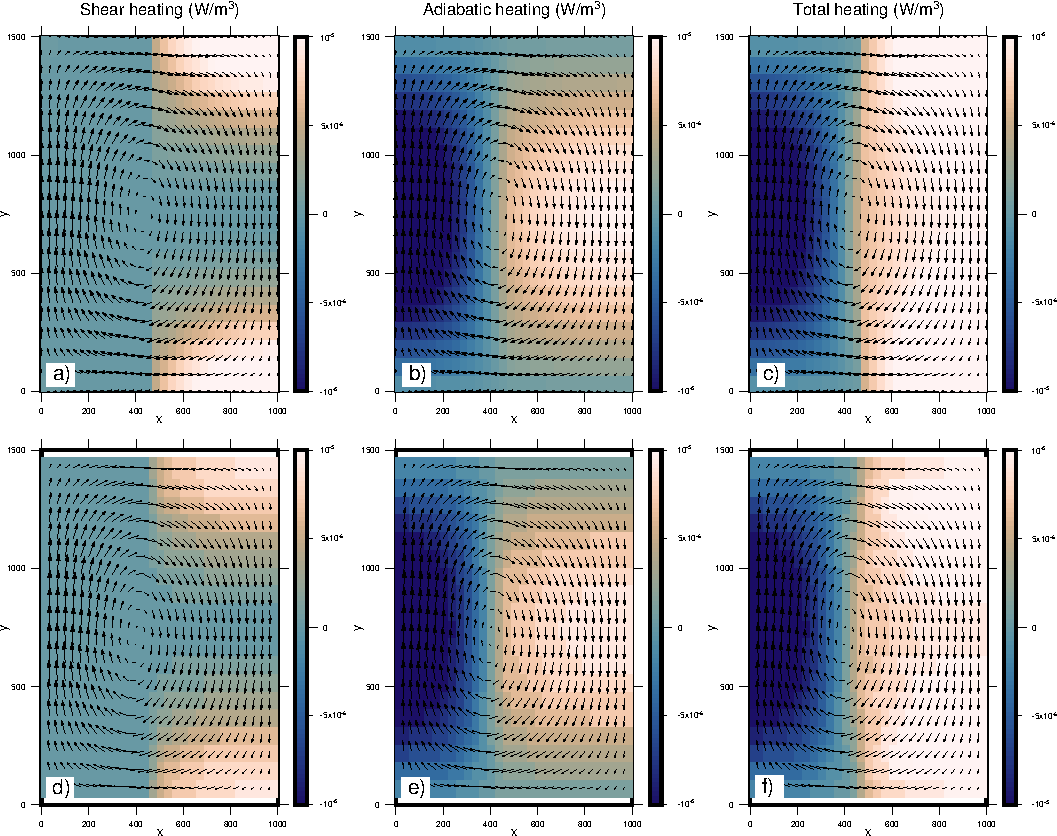
\includegraphics[width=400px]{./Figures/Energy.pdf}
\caption{Comparison between shear (first column), adiabatic (second column) and total (third column) energy predicted by the code (panels a, b and c) and those
created using example ${Shear\_adiabatic\_heating.m}$ from Exercise 9.4 in \citet{Gerya2010} (panels d, e and f).}
\label{fig:energy}
\end{figure}